%%%%%%%%%%%%%%%%%%%%%%%%%%%%%%%%%%%%%%%%%
% Classicthesis-Styled CV
% LaTeX Template
% Version 1.0 (22/2/13)
%
% This template has been downloaded from:
% http://www.LaTeXTemplates.com
%
% Original author:
% Alessandro Plasmati
%
% License:
% CC BY-NC-SA 3.0 (http://creativecommons.org/licenses/by-nc-sa/3.0/)
%
%%%%%%%%%%%%%%%%%%%%%%%%%%%%%%%%%%%%%%%%%

%----------------------------------------------------------------------------------------
%	PACKAGES AND OTHER DOCUMENT CONFIGURATIONS
%----------------------------------------------------------------------------------------

\documentclass[10pt,a4paper]{scrartcl}

\reversemarginpar % Move the margin to the left of the page 

\newcommand{\MarginText}[1]{\marginpar{\raggedleft\itshape\small#1}} % New command defining the margin text style

\usepackage[dvipsnames]{xcolor}
\usepackage[nochapters]{classicthesis} % Use the classicthesis style for the style of the document
\usepackage[LabelsAligned]{currvita} % Use the currvita style for the layout of the document
\usepackage{graphicx}
\usepackage{caption}
\usepackage{wrapfig}
\usepackage[left=5cm,right=2.3cm,top=2cm,bottom=2cm]{geometry}

\hypersetup{pdftitle={CVCeciliaDiMaulo},
    pdfauthor={Cecilia.DiMaulo},
    pdfsubject={},
    pdfkeywords={},
    colorlinks=false,       % no lik border color
    allbordercolors=white    % white border color for all
}


\renewcommand{\cvheadingfont}{\LARGE\color{RubineRed}} % Font color of your name at the top


\usepackage{hyperref} % Required for adding links	and customizing them
\hypersetup{colorlinks, breaklinks, urlcolor=RubineRed, linkcolor=RubineRed} % Set link colors

\newlength{\datebox}\settowidth{\datebox}{10.2018-1.2018} % Set the width of the date box in each block

\newcommand{\NewEntryL}[3]{\noindent\hangindent=2em\hangafter=0 \parbox{\datebox}{\normalsize \textit{#1}}\hspace{5em} #2 #3 % Define a command for each new block - change spacing and font sizes here: #1 is the left margin, #2 is the italic date field and #3 is the position/employer/location field
\vspace{0.5em}} % Add some white space after each new entry

\newcommand{\NewEntry}[3]{\noindent\hangindent=2em\hangafter=0 \parbox{\datebox}{\normalsize \textit{#1}}\hfill\spacedlowsmallcaps{#2} #3 % Define a command for each new block - change spacing and font sizes here: #1 is the left margin, #2 is the italic date field and #3 is the position/employer/location field
\vspace{0.5em}} % Add some white space after each new entry

\newcommand{\Description}[1]{\hangindent=2em\hangafter=0\raggedright\footnotesize{#1}\par\normalsize\vspace{1em}} % Define a command for descriptions of each entry - change spacing and font sizes here

%----------------------------------------------------------------------------------------

\begin{document}

\thispagestyle{empty} % Stop the page count at the bottom of the first page

%----------------------------------------------------------------------------------------
%	NAME AND CONTACT INFORMATION SECTION
%----------------------------------------------------------------------------------------

\begin{wrapfigure}{L}{1em}
 \hspace*{-10em}
 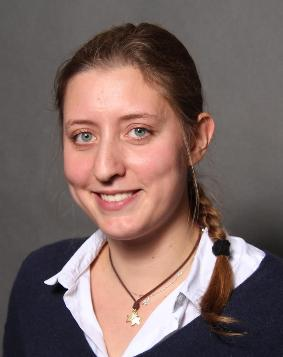
\includegraphics[scale=0.3]{img/ceci.jpg}
\end{wrapfigure}

\begin{cv}{\spacedallcaps{Cecilia Di Maulo} \ \ \ \ \ \ \  \large\emph{25 ans}}\vspace{2em} % Your name

%\begin{wrapfigure}{License{1em}
% \hspace*{-10em}
% 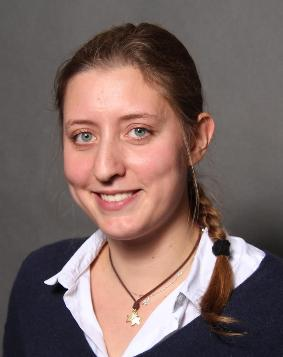
\includegraphics[scale=0.3]{img/ceci.jpg}
%\end{wrapfigure}

\NewEntryL{email}{\href{mailto:cecidimaulo@gmail.com}{cecidimaulo@gmail.com}} % Email address

\NewEntryL{t\'{e}l\'{e}phone}{ +33 6 26 30 86 90} % Phone number(s)

\NewEntryL{adresse}{ 4, rue du vieil abreuvoir, Saint-Germain-en-Laye} % Phone number(s)

\vspace{1.2em} % Extra white space betweelinksn the personal information section and goal

%\noindent\spacedlowsmallcaps{Goal}\vspace{1em} % Goal heading, could be used for a quotation or short profile instead

%\Description{Gain fundamental experience in my area of interest and expertise.}\vspace{2em} % Goal text

  \fcolorbox{white}{RubineRed}{\parbox{\dimexpr\textwidth-2\fboxsep-2\fboxrule}{\tiny\textcolor{white}{\hspace{1.5 cm}}}}

\vspace{1.5em} % Extra white space betweelinksn the personal information section and goal
%----------------------------------------------------------------------------------------
%	WORK EXPERIENCE
%----------------------------------------------------------------------------------------

  \noindent\color{RubineRed}\spacedallcaps{Exp\'eriences de travail}\vspace{1em}

  \color{black} \NewEntry{05.2018-...}{Ing\'{e}nieur de Production Cloud Computing}

  \Description{\MarginText{Osones}Mission \`{a} l'IRT SystemX : mise \`{a} jour du IaaS de production bas\'e sur OpenStack
        \begin{itemize}
          \item {Mont\'{e}e de 4 versions d'OpenStack (9 serveurs)} 
        \item {Int\'{e}gration d'un service de gestion de volumes additionnels pour les VMs}
        \item {Int\'{e}gration d'un service de Load Balancing}
        \item {Int\'{e}gration d'un service de m\'{e}trologie pour les VMs}
        \end{itemize}
    \emph{technologies utilis\'{e}es : OpenStack-Ansible, Ubuntu 14.04 \& 16.04, Ansible, Terraform, iSCSI}
  }
%------------------------------------------------

  \NewEntry{10.2017-4.2018}{Ing\'{e}nieur R\&D en cybers\'{e}curit\'{e}}

  \Description{\MarginText{Thal\`{e}s Services}\'Evaluation de services d'orchestration de VNFs    
        \begin{itemize}
          \item {\'{E}tude et comparaison de services d'orchestration de VNFs}
          \item {Conception de l'architecture d'une plateforme 5G bas\'{e}e sur OpenStack}
        \end{itemize}
  }

%------------------------------------------------

\NewEntry{02-08.2017}{Stage fin d'\'etudes orient\'e Recherche}

\Description{\MarginText{Orange Labs Networks}\'Etude de la supervision des r\'eseaux 5G pour les cas d'usage de l'IOT}

%------------------------------------------------

\vspace{2em} % Extra space between major sections

%----------------------------------------------------------------------------------------
%	EDUCATION
%----------------------------------------------------------------------------------------

\color{RubineRed}\spacedallcaps{\'Etudes et Formations}\vspace{1em}


\color{black}
\NewEntry{2017}{Master Computer science for Communication Networks}

\Description{\MarginText{Universit\'e de Paris Saclay} 
\textbf{Projet de fin d'\'etudes:} \textit{OSes for Cyber Physical Systems}, \'etat de l'art et \'etude des performances.}

%------------------------------------------------

\NewEntry{2014 - 2017}{Dipl\^ome d'ing\'enieur g\'en\'eraliste T\'el\'ecoms}

\Description{\MarginText{T\'el\'ecom SudParis, Evry}\textbf{Projet de groupe de premi\`ere ann\'ee} avec la start up Auticiel: "Introduire la tablette en EHPAD": \emph{Gestion de Projet, Test, R\'edaction de Tutoriels}\newline
    \textbf{Projet de groupe d'informatique de premi\`ere ann\'ee}:
    "Jeu de plateforme Mario-like": \emph{langage C (librairie graphique SDL), Tile-Mapping, Git}} 

%------------------------------------------------

\NewEntry{03-08.2016}{Semestre d'\'echange universitaire}

\Description{\MarginText{Universidade Federal do Ceara, Fortaleza, Brazil}\emph{Mati\`eres principales : D\'eveloppement logiciel pour le Cloud (AWS), Web S\'emantique, Logique Floue, Intelligence Artificielle}} 

%------------------------------------------------

\NewEntry{2011 - 2014}{Classe pr\'eparatoire aux grandes \'ecoles}

\Description{\MarginText{Lyc\'ee Pasteur, Neuilly-sur-Seine}} 

%------------------------------------------------
\NewEntry{2011}{Baccalaur\'eat International Scientifique}

\Description{\MarginText{Lyc\'ee International, St-Germain-en-Laye}\textbf{Dipl\^ome franco-italien} option Math\'ematiques. \emph{Mention Tr\`es Bien}} 

%------------------------------------------------
\vspace{22em} % Extra space between major sections

%----------------------------------------------------------------------------------------
%	OTHER INFORMATION
%----------------------------------------------------------------------------------------
\color{RubineRed}
\spacedallcaps{Informations Suppl\'ementaires}\vspace{1em}

\vspace{1em}

\color{black}
\newlength{\langbox} % Create a new length for the length of languages to keep them equally spaced
\settowidth{\langbox}{Francais} % Length equals the length of "English" - if you have a longer language in your list put it here

\Description{\MarginText{Langues}\parbox{\langbox}{\textsc{Italien}}\ \ $\cdotp$\ \ \ C2 - Langue Maternelle}

\vspace{-0.5em} % Negative vertical space to counteract the vertical space between every \Description command

\Description{\parbox{\langbox}{\textsc{Francais}}\ \ $\cdotp$\ \ \ C2 - Langue Maternelle}  

\vspace{-0.5em} % Negative vertical space to counteract the vertical space between every \Description command

\Description{\parbox{\langbox}{\textsc{Anglais}}\ \ $\cdotp$\ \ \ C2}

\vspace{-0.5em} % Negative vertical space to counteract the vertical space between every \Description command

\Description{\parbox{\langbox}{\textsc{Portugais}}\ \ $\cdotp$\ \ \ C1}

\vspace{1em} % Negative vertical space to counteract the vertical space between every \Description command

%------------------------------------------------

\Description{\MarginText{Int\'er\^ets}\textbf{Volley-ball} (niveau Nationale 3  en 2009-2013),
    \textbf{Plong\'ee} (Dipl\^ome Rescue Diver),
    \textbf{Ski} (9 ann\'ees de slalom g\'eant, puis 5 ann\'ees de freestyle)
    \textbf{Lectrice passionn\'ee} (Oeuvres classiques Italiennes, Francaises et Anglaises en langue originale),
    \textbf{Voyage},
    \textbf{Piano et Saxophone}}
%----------------------------------------------------------------------------------------
\date{}
\end{cv}

\end{document}
